\documentclass{article}
\usepackage{tikz}
\usetikzlibrary{patterns}
\usepackage{subcaption}
\usepackage[margin=0.5in]{geometry}

\begin{document}

\begin{figure}[ht]
    \centering
    \begin{subfigure}{0.32\textwidth}
        \centering
        \resizebox{\textwidth}{!}{\input{corr_view_a.tex}}
        \caption{Syndrome and Errors}
    \end{subfigure}
    \hfill
    \begin{subfigure}{0.32\textwidth}
        \centering
        \resizebox{\textwidth}{!}{\input{corr_view_b.tex}}
        \caption{Matching in $\mathcal{R}
    \end{subfigure}
    \hfill
    \begin{subfigure}{0.32\textwidth}
        \centering
        \resizebox{\textwidth}{!}{\input{corr_view_c.tex}}
        \caption{Matching in $\mathcal{R}
    \end{subfigure}
    \vspace{0.5cm}
    \begin{subfigure}{0.32\textwidth}
        \centering
        \resizebox{\textwidth}{!}{\input{corr_view_d.tex}}
        \caption{Logical Error (Restriction)}
    \end{subfigure}
    \hfill
    \begin{subfigure}{0.32\textwidth}
        \centering
        \resizebox{\textwidth}{!}{\input{corr_view_g.tex}}
        \caption{Matching in $\mathcal{R}
    \end{subfigure}
    \hfill
    \begin{subfigure}{0.32\textwidth}
        \centering
        \resizebox{\textwidth}{!}{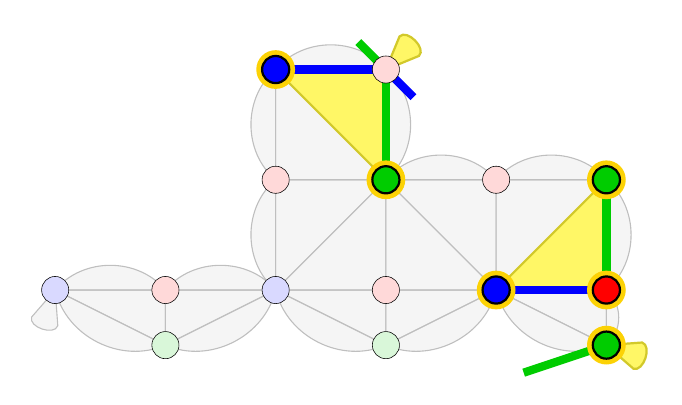
\begin{tikzpicture}[scale=0.35]
    \filldraw[fill=gray!15, draw=gray!50, , fill opacity=0.5] (5,1) -- (5,3) -- (1,3) -- cycle;
    \filldraw[fill=gray!15, draw=gray!50, , fill opacity=0.5] (5,3) to[bend right=50] (1,3) -- cycle;
    \filldraw[fill=gray!15, draw=gray!50, , fill opacity=0.5] (5,1) -- (9,3) -- (5,3) -- cycle;
    \filldraw[fill=gray!15, draw=gray!50, , fill opacity=0.5] (5,3) to[bend left=50] (9,3) -- cycle;
    \filldraw[fill=gray!15, draw=gray!50, , fill opacity=0.5] (13,1) -- (13,3) -- (9,3) -- cycle;
    \filldraw[fill=gray!15, draw=gray!50, , fill opacity=0.5] (9,3) -- (13,3) -- (13,7) -- cycle;
    \filldraw[fill=gray!15, draw=gray!50, , fill opacity=0.5] (13,1) -- (17,3) -- (13,3) -- cycle;
    \filldraw[fill=gray!15, draw=gray!50, , fill opacity=0.5] (13,3) -- (17,3) -- (13,7) -- cycle;
    \filldraw[fill=gray!15, draw=gray!50, , fill opacity=0.5] (21,1) -- (21,3) -- (17,3) -- cycle;
    \filldraw[fill=gray!15, draw=gray!50, , fill opacity=0.5] (21,3) to[bend left=50] (21,1) -- cycle;
    \filldraw[fill=gray!15, draw=gray!50, , fill opacity=0.5] (21,3) to[bend right=50] (21,7) -- cycle;
    \filldraw[fill=gray!15, draw=gray!50, , fill opacity=0.5] (9,7) to[bend right=50] (9,3) -- cycle;
    \filldraw[fill=gray!15, draw=gray!50, , fill opacity=0.5] (9,7) to[bend left=50] (9,11) -- cycle;
    \filldraw[fill=gray!15, draw=gray!50, , fill opacity=0.5] (9,3) -- (13,7) -- (9,7) -- cycle;
    \filldraw[fill=gray!15, draw=gray!50, , fill opacity=0.5] (9,7) -- (13,7) -- (9,11) -- cycle;
    \filldraw[fill=gray!15, draw=gray!50, , fill opacity=0.5] (17,3) -- (17,7) -- (13,7) -- cycle;
    \filldraw[fill=gray!15, draw=gray!50, , fill opacity=0.5] (17,7) to[bend right=50] (13,7) -- cycle;
    \filldraw[fill=gray!15, draw=gray!50, , fill opacity=0.5] (17,3) -- (21,7) -- (17,7) -- cycle;
    \filldraw[fill=gray!15, draw=gray!50, , fill opacity=0.5] (17,7) to[bend left=50] (21,7) -- cycle;
    \filldraw[fill=gray!15, draw=gray!50, , fill opacity=0.5] (13,11) to[bend right=50] (9,11) -- cycle;
    \filldraw[fill=gray!15, draw=gray!50, , fill opacity=0.5] (13,11) to[bend left=50] (13,7) -- cycle;
    \filldraw[fill=gray!15, draw=gray!50, , fill opacity=0.5] (9,3) to[bend left=50] (5,1) -- cycle;
    \filldraw[fill=gray!15, draw=gray!50, , fill opacity=0.5] (9,3) to[bend right=50] (13,1) -- cycle;
    \filldraw[fill=gray!15, draw=gray!50, , fill opacity=0.5] (17,3) to[bend left=50] (13,1) -- cycle;
    \filldraw[fill=gray!15, draw=gray!50, , fill opacity=0.5] (17,3) to[bend right=50] (21,1) -- cycle;
    \filldraw[fill=gray!15, draw=gray!50, , fill opacity=0.5] (1,3) -- (1.095,1.703) to[bend left=90] (0.146,2.020) -- cycle;
    \filldraw[fill=gray!15, draw=gray!50, , fill opacity=0.5] (1,3) to[bend right=50] (5,1) -- cycle;
    \filldraw[fill=yellow!60, draw=yellow!80!black, thick, , fill opacity=1.0] (17,3) -- (21,3) -- (21,7) -- cycle;
    \filldraw[fill=yellow!60, draw=yellow!80!black, thick, , fill opacity=1.0] (13,7) -- (13,11) -- (9,11) -- cycle;
    \filldraw[fill=yellow!60, draw=yellow!80!black, thick, , fill opacity=1.0] (13,11) -- (13.495,12.202) to[bend left=90] (14.202,11.495) -- cycle;
    \filldraw[fill=yellow!60, draw=yellow!80!black, thick, , fill opacity=1.0] (21,1) -- (22.297,1.095) to[bend left=90] (21.980,0.146) -- cycle;
    \draw[blue, line width=3pt] (21.0, 3.0) -- (17.0, 3.0);
    \draw[blue, line width=3pt] (13.0, 11.0) -- (14, 10);
    \draw[blue, line width=3pt] (13.0, 11.0) -- (9.0, 11.0);
    \draw[green!80!black, line width=3pt] (21.0, 3.0) -- (21.0, 7.0);
    \draw[green!80!black, line width=3pt] (13.0, 11.0) -- (13.0, 7.0);
    \draw[green!80!black, line width=3pt] (13.0, 11.0) -- (12, 12);
    \draw[green!80!black, line width=3pt] (21.0, 1.0) -- (18, 0);
    \filldraw[fill=red!15, draw=black, very thin] (5.0, 3.0) circle (14pt);
    \filldraw[fill=red!15, draw=black, very thin] (13.0, 3.0) circle (14pt);
    \filldraw[fill=yellow!70!orange, draw=none] (21.0, 3.0) circle (20pt);
    \filldraw[fill=red, draw=black, thick] (21.0, 3.0) circle (14pt);
    \filldraw[fill=red!15, draw=black, very thin] (9.0, 7.0) circle (14pt);
    \filldraw[fill=red!15, draw=black, very thin] (17.0, 7.0) circle (14pt);
    \filldraw[fill=red!15, draw=black, very thin] (13.0, 11.0) circle (14pt);
    \filldraw[fill=blue!15, draw=black, very thin] (9.0, 3.0) circle (14pt);
    \filldraw[fill=yellow!70!orange, draw=none] (17.0, 3.0) circle (20pt);
    \filldraw[fill=blue, draw=black, thick] (17.0, 3.0) circle (14pt);
    \filldraw[fill=yellow!70!orange, draw=none] (13.0, 7.0) circle (20pt);
    \filldraw[fill=green!80!black, draw=black, thick] (13.0, 7.0) circle (14pt);
    \filldraw[fill=blue!15, draw=black, very thin] (1.0, 3.0) circle (14pt);
    \filldraw[fill=yellow!70!orange, draw=none] (9.0, 11.0) circle (20pt);
    \filldraw[fill=blue, draw=black, thick] (9.0, 11.0) circle (14pt);
    \filldraw[fill=yellow!70!orange, draw=none] (21.0, 7.0) circle (20pt);
    \filldraw[fill=green!80!black, draw=black, thick] (21.0, 7.0) circle (14pt);
    \filldraw[fill=green!80!black!15, draw=black, very thin] (5.0, 1.0) circle (14pt);
    \filldraw[fill=green!80!black!15, draw=black, very thin] (13.0, 1.0) circle (14pt);
    \filldraw[fill=yellow!70!orange, draw=none] (21.0, 1.0) circle (20pt);
    \filldraw[fill=green!80!black, draw=black, thick] (21.0, 1.0) circle (14pt);
\end{tikzpicture}}
        \caption{Success (Correlated)}
    \end{subfigure}
    
    \vspace{0.5cm}
    \caption{Syndrome and Errors}
\end{figure}

\end{document}